\documentclass{mwrep}
\usepackage{polski}
\usepackage[polish]{babel}
\usepackage[utf8]{inputenc}
\usepackage{tgbonum}
\usepackage{graphicx}
\usepackage{tabularx}
\usepackage{hyperref}

\makeatletter
\let\ps@closing\ps@plain
\makeatother

\renewcommand{\labelitemi}{$\bullet$}
\setlength{\parindent}{0cm}
\addto\captionspolish{\renewcommand{\tablename}{Tabela}}

\newcommand*{\titleGP}{\begingroup
\centering

{\large Studencka Pracownia Inżynierii Oprogramowania}\\Instytut Informatyki Uniwersytetu Wrocławskiego\par
\vspace*{16\baselineskip}

{\Large Rafał Hirsz, Karol Wieczorek, Krzysztof Wróbel\par}
\vspace*{\baselineskip}

\rule{\textwidth}{1.6pt}\vspace*{-\baselineskip}\vspace*{2pt}
\rule{\textwidth}{0.4pt}\\[\baselineskip]

{\Huge SYMULATOR LOTU}\\[0.2\baselineskip]

\rule{\textwidth}{0.4pt}\vspace*{-\baselineskip}\vspace{3.2pt}
\rule{\textwidth}{1.6pt}\\[\baselineskip]

\scshape
{\huge Architektura oprogramowania}\par
\vspace*{2\baselineskip}

\begin{figure}[h]
\centering

\includegraphics[width=5\baselineskip]{flightsim-team-logo.pdf}
\end{figure}
\vfill

{\large Wrocław 2014}\par

\pagebreak

\endgroup}

\begin{document}

\thispagestyle{empty}
\titleGP

\begin{center}
\begin{table}[h]
\begin{center}
\caption{Historia zmian dokumentu}\label{T:Zmiany}
\vspace{3ex}
\begin{tabularx}{1\textwidth}{|l|l|l|X|}
\hline
Data & Wersja & Autor & Opis zmian \\ \hline
2014-01-21 & 1.0 & Rafał Hirsz & Utworzenie dokumentu \\
\hline
\end{tabularx}
\end{center}
\end{table}
\end{center}

\pagebreak

\tableofcontents

\chapter{Ogólny opis architektury}

Kod źródłowy \textit{Symulatora lotu} zostanie napisany w~języku C++. W~celu zapewnienia płynności rozgrywki zostanie wykorzystana biblioteka OpenGL, pozwalająca na~pełne wykorzystanie możliwości nowoczesnych kart graficznych. Motywacją do~wyboru tych narzędzi jest ich dojrzałość, duże możliwości dostosowania do potrzeb oraz popularność wśród programistów.

\vspace{1em}
\textit{Symulator lotu} będzie składał się z następujących modułów:
\begin{itemize}
    \item mechanizmu graficznego,
    \item symulatora dynamiki newtonowskiej,
    \item systemu czytania zasobów graficznych,
    \item interfejsu użytkownika,
    \item środowiska symulacji.
\end{itemize}

\vspace{1em}
Zależności pomiędzy poszczególnymi modułami są opisane na rysunku \ref{F:zaleznosci}.

\begin{figure}[h]
\centering
\caption{Diagram zależności pomiędzy modułami \textit{Symulatora lotu} \label{F:zaleznosci}}
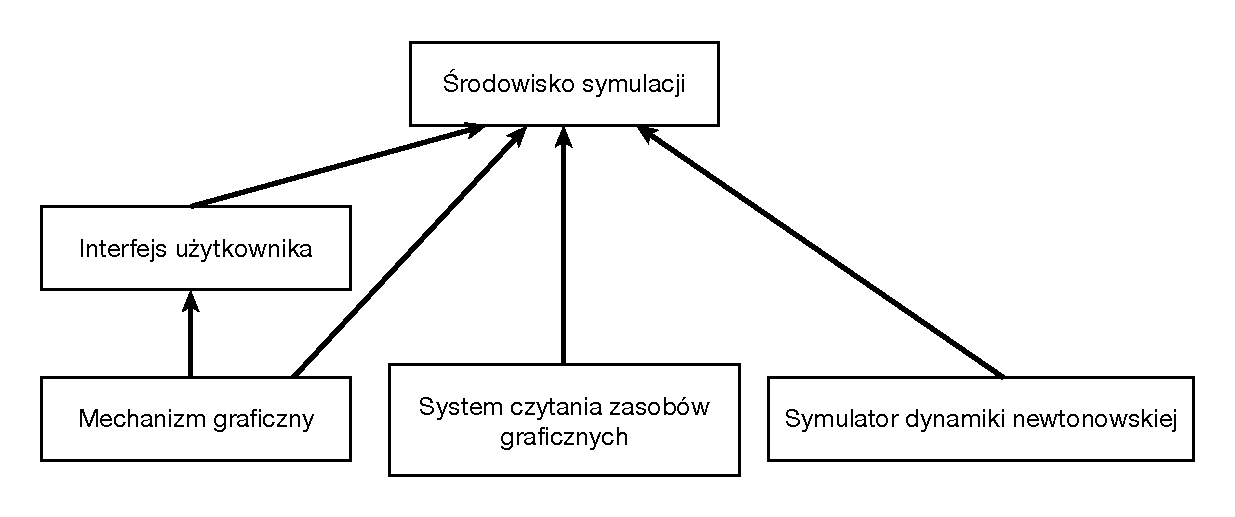
\includegraphics[width=\textwidth]{diagram-zaleznosci-ai.pdf}
\end{figure}

\section{Mechanizm graficzny}
Mechanizm graficzny jest podstawową jednostką odpowiedzialną za~wyświetlanie obrazu na~ekranie. Pozwala na~wygodne zarządzanie obiektami na~trójwymiarowej scenie oraz ich przedstawienie w~postaci pikseli w~wydajny sposób. Dodatkową możliwością jest zastosowanie efektów znacząco poprawiających jakość obrazu, takich jak teselacja\footnotemark[1]{}. Mechanizm graficzny będzie podstawą, na~której opierać się będą pozostałe komponenty związane w~jakikolwiek sposób z~wyświetlaniem grafiki.

\footnotetext[1]{Patrz \cite{zalozenia}, \textit{Słownik pojęć}}

\section{Symulator dynamiki newtonowskiej}
Symulator dynamiki newtonowskiej pozwala na~przeprowadzenie obliczeń związanych z~zachowaniem się obiektów w~trójwymiarowej przestrzeni zgodnym z rzeczywistością. Moduł ten będzie napisany z~uwzględnieniem szczególnej dokładności wyników obliczeń potrzebnej do~odwzorowania wszystkich aspektów symulacji lotu.

\section{System czytania zasobów graficznych}
System czytania zasobów graficznych rozszerza silnik graficzny o~możliwość użycia zewnętrznych grafik i~modeli w symulatorze. Pozwala on~grafikom na~wygodne tworzenie zasobów w~zewnętrznych programach, zapewniając obsługę popularnych formatów graficznych: OpenEXR, PNG, OBJ, COLLADA. System ten będzie napisany w~sposób modułowy w~celu umożliwienia łatwej rozbudowy go o~obsługę innych formatów.

\section{Interfejs użytkownika}
Interfejs użytkownika używa mechanizmu graficznego do~narysowania elementów składowych interfejsu użytkownika, takich~jak przyciski, etykiety, czy pola tekstowe, oraz obsługi klawiatury i~myszy. Będzie~to osobny moduł, zależny jedynie od~mechanizmu graficznego.

\section{Środowisko symulacji}
Środowisko sytuacji łączy pozostałe moduły, umożliwiając faktyczną rozgrywkę opisaną w~\cite{zalozenia}. Tutaj będą wdrożone zasady rozgrywki oraz~przejścia pomiędzy poszczególnymi ekranami interfejsu użytkownika.

\chapter{Architektura a wymagania}

\section{Realizm}
Zastosowanie biblioteki OpenGL pozwala na~precyzyjną kontrolę nad wyświetlaniem obrazu. Dzięki temu możliwe jest zastosowanie zaawansowanych technik poprawiających jakość grafiki. Dodatkowo użycie zewnętrznych zasobów graficznych, znacznie ułatwia osiągnięcie realizmu graficznego. Realizm symulacji fizycznej osiągnięty zostanie dzięki wysokiej dokładności obliczeń symulatora dynamiki newtonowskiej.

\section{Niezawodność}
Moduły \textit{Symulatora lotu} stworzone zostaną przy użyciu języka C++ oraz biblioteki OpenGL. Narzędzia te pozwalają na~drobiazgową kontrolę nad każdym aspektem działania symulatora, poczynając od~kontroli pamięci, a~kończąc na~wyświetlaniu grafiki. Skorzystanie z nich pozwala na sprawdzenie poprawności kodu odpowiadającego za każdy poziom działania symulatora, co gwarantuje jego niezawodność.

\begin{thebibliography}{9}
    \bibitem{zalozenia} R. Hirsz, K. Wieczorek, K. Wróbel: \textit{Symulator lotu: Założenia ogólne}, Wrocław, SPIO IIUWr 2014.
\end{thebibliography}

\end{document}